\documentclass[conference]{IEEEtran}
\usepackage[T1]{fontenc}
\usepackage{graphicx}
\usepackage{booktabs}
\usepackage{amsmath}
\usepackage{cite}
\usepackage{xcolor}
\usepackage[hidelinks]{hyperref}
\graphicspath{{figures/}}

% All numbers below come from results/ via scripts/make_paper_assets.py
% AUTO-GENERATED by scripts/make_paper_assets.py from results/ -- do not edit by hand
\newcommand{\vEoneMOTA}{76.6}
\newcommand{\vEoneIDF}{79.3}
\newcommand{\vEoneIDs}{164}
\newcommand{\vEoneHOTA}{67.9}
\newcommand{\vEoneDetA}{66.6}
\newcommand{\vEoneAssA}{69.8}
\newcommand{\vInterpMOTA}{78.3}
\newcommand{\vInterpIDF}{80.2}
\newcommand{\vMatchEightMOTA}{76.4}
\newcommand{\vMatchEightIDF}{79.0}
\newcommand{\vMatchEightIDs}{202}
\newcommand{\vFpThirtyTwoMOTA}{76.6}
\newcommand{\vFpThirtyTwoIDF}{78.7}
\newcommand{\vSortMOTA}{74.6}
\newcommand{\vSortIDF}{77.2}
\newcommand{\vSortIDs}{287}
\newcommand{\vDetMsFP}{58}
\newcommand{\vDetMsFPthirtytwo}{107}
\newcommand{\vStaticHOTA}{71.2}
\newcommand{\vStaticDetA}{69.4}
\newcommand{\vStaticAssA}{73.5}
\newcommand{\vStaticIDF}{82.6}
\newcommand{\vStaticShareGT}{69}
\newcommand{\vStaticShareIDSW}{52}
\newcommand{\vStaticIDSWk}{2.4}
\newcommand{\vMovingHOTA}{60.3}
\newcommand{\vMovingDetA}{60.9}
\newcommand{\vMovingAssA}{60.1}
\newcommand{\vMovingIDF}{73.7}
\newcommand{\vMovingShareGT}{31}
\newcommand{\vMovingShareIDSW}{48}
\newcommand{\vMovingIDSWk}{4.8}
\newcommand{\vGapHOTA}{10.9}
\newcommand{\vGapDetA}{8.4}
\newcommand{\vGapAssA}{13.4}
\newcommand{\vGapMin}{9.8}
\newcommand{\vGapMax}{12.6}
\newcommand{\vMotionStaticMax}{0.003}
\newcommand{\vMotionMovingMin}{0.18}
\newcommand{\vMotionMovingMax}{0.70}
\newcommand{\vRhoMovMin}{-0.43}
\newcommand{\vRhoMovMax}{-0.25}
\newcommand{\vRhoStatMin}{-0.22}
\newcommand{\vRhoStatMax}{-0.12}
\newcommand{\vErrLow}{0.011}
\newcommand{\vErrHigh}{0.047}
\newcommand{\vRhoFlowErr}{0.51}
\newcommand{\vNMatches}{44{,}507}
\newcommand{\vFitOkMin}{92}
\newcommand{\vLostStatic}{6.0}
\newcommand{\vLostMoving}{2.1}
\newcommand{\vLostIoUStatic}{0.27}
\newcommand{\vLostIoUMoving}{0.10}
\newcommand{\vLostRhoWithin}{0.00}
\newcommand{\vLostRhoPooled}{-0.15}
\newcommand{\vHighSw}{41}
\newcommand{\vLowSw}{39}
\newcommand{\vHighSwk}{4.98}
\newcommand{\vLowSwk}{4.61}
\newcommand{\vHighIoU}{0.83}
\newcommand{\vLowIoU}{0.86}

\newcommand{\repocommit}{b73239e}

\begin{document}

\title{ByteTrack Under Camera Motion:\\ Reproduction and Error Analysis on MOT17}

\author{\IEEEauthorblockN{Vanodhya Warnasooriya}
\IEEEauthorblockA{Department of Electrical Engineering, Chulalongkorn University, Bangkok, Thailand\\
Student ID 6872086821 \quad 2102515 Digital Video Processing, Semester 1/2026}}

\maketitle

\begin{abstract}
ByteTrack predicts every track with a constant-velocity Kalman filter in image coordinates, so a moving camera
appears to the filter as motion of every person. We reproduce ByteTrack on the MOT17 half-validation split with the
official code and weights and obtain \vEoneMOTA{} MOTA and \vEoneIDF{} IDF1, equal to the published values. We then
split the error by camera type. The four moving-camera sequences hold \vMovingShareGT\% of the ground-truth boxes but
\vMovingShareIDSW\% of the identity switches, and their HOTA is \vGapHOTA{} points lower than on static cameras, a gap
that stays between \vGapMin{} and \vGapMax{} points under six tracker and detector settings. The loss is larger in
association (AssA $-$\vGapAssA) than in detection (DetA $-$\vGapDetA). A per-frame estimate of global motion (ORB
features and a RANSAC fit) shows that camera motion degrades the one-frame Kalman prediction, but the predicted box
still overlaps its detection well enough to be matched. The penalty appears when a lost track must be re-found: after
9--16 lost frames, \vLostMoving\% of lost tracks are recovered with a moving camera against \vLostStatic\% with a static
one.
\end{abstract}

\begin{IEEEkeywords}
multi-object tracking, ByteTrack, Kalman filter, camera motion, reproducibility, MOT17
\end{IEEEkeywords}

% =====================================================================================================
\section{Introduction}
Tracking-by-detection links the boxes of a detector over time. ByteTrack~\cite{zhang2022bytetrack} is a strong and
simple example: a YOLOX detector~\cite{ge2021yolox} gives boxes, a Kalman filter~\cite{kalman1960} predicts where each
track will be in the next frame, and the boxes are matched to the predictions by intersection over union (IoU). Its
key idea, BYTE, also matches low-score boxes in a second step, which recovers people who are partly occluded.

The Kalman filter assumes constant velocity \emph{in image coordinates}. When the camera pans, walks or drives, every
person moves in the image even if they stand still. About half of the MOT17 sequences are filmed with a moving
camera~\cite{milan2016mot16}, but the ByteTrack paper reports only results averaged over all sequences. It is therefore
not known how much of ByteTrack's error comes from camera motion, and through which part of the tracker.

This Level~A study reproduces ByteTrack and analyses its error by camera type. Our contributions are:
\begin{itemize}
\item a reproduction of ByteTrack on MOT17 half-val that matches the published MOTA and IDF1, together with an
explanation of the setting behind the published numbers (Sec.~\ref{sec:e1});
\item a split of the error into static- and moving-camera sequences, which shows a stable gap of about
\vGapHOTA{} HOTA points, mainly in association (Sec.~\ref{sec:e2});
\item a per-frame mechanism study that relates measured camera motion to the Kalman prediction and locates the loss in
the recovery of lost tracks (Sec.~\ref{sec:e3}), and a sensitivity study showing that the gap persists across
tracker settings (Sec.~\ref{sec:e4}).
\end{itemize}

% =====================================================================================================
\section{Related Work}
\textbf{Motion-based association.} SORT~\cite{bewley2016sort} introduced the Kalman filter plus IoU and Hungarian
matching that ByteTrack still uses; its motion model is explicitly independent of camera motion. DeepSORT~\cite{wojke2017deepsort}
added appearance features and the 8-D box state that ByteTrack inherits. ByteTrack~\cite{zhang2022bytetrack} keeps
the motion model and changes which detections are associated; it reports that the Kalman filter fails on BDD100K
because of large camera motion, but gives no per-camera breakdown on MOT17.
\textbf{Camera motion compensation.} BoT-SORT~\cite{aharon2022botsort} adds global motion compensation to ByteTrack and
improves IDF1 by 1.6 points on MOT17 half-val, but it reports only overall numbers and does not show where the gain
comes from. OC-SORT~\cite{cao2023ocsort} shows that Kalman errors accumulate while a track has no observation, but it
studies occlusion and non-linear motion, not the camera.
\textbf{Metrics.} MOTA~\cite{bernardin2008clear} is dominated by detection errors and IDF1~\cite{ristani2016idf1} by
identity errors; HOTA~\cite{luiten2021hota} separates detection (DetA) from association (AssA), which we use to locate
the loss.

% =====================================================================================================
\section{Experimental Setup}
\textbf{Data and split.} We use the seven MOT17 training sequences (FRCNN copies) and the half split of
ByteTrack~\cite{zhang2022bytetrack}: the first half of each sequence was used for training, the second half
(2{,}652 frames) for evaluation. Following the MOT16/17 benchmark table~\cite{milan2016mot16}, MOT17-02, 04 and 09 are
static-camera sequences and MOT17-05, 10, 11 and 13 are moving-camera sequences.

\textbf{Baseline.} We run the official ByteTrack code (commit \texttt{d1bf019}) with its \texttt{ByteTrack\_ablation}
weights (YOLOX-X trained on CrowdHuman and the first half of MOT17), input $800\times1440$, FP16 inference, and the
default tracker settings of \texttt{tools/track.py}: high-score threshold 0.6, matching threshold 0.9, and a lost-track
buffer of 30 frames (14 for MOT17-05 and 25 for MOT17-13, as hard-coded in the official evaluator). The tracker code is
unchanged; a small compatibility layer only replaces a compiled IoU routine with an equivalent NumPy version. Detections
are computed once and cached, so every tracker variant uses identical boxes.

\textbf{Metrics.} We report MOTA, IDF1 and ID switches with ByteTrack's own evaluation (py-motmetrics, marked $^*$) for a
direct comparison with the paper, and HOTA, DetA and AssA with TrackEval~\cite{luiten2021hota}.

\textbf{Camera motion.} For each frame pair we detect up to 3{,}000 ORB features~\cite{rublee2011orb} on a 960-pixel-wide
grey image, mask out the detector's own person boxes, match the features with a ratio test, and fit a similarity
transform $A_t$ (rotation, scale, translation) with RANSAC~\cite{fischler1981ransac}. Camera motion is the mean
displacement of the four image corners under $A_t$, in percent of the image diagonal per frame. The fit succeeds in at
least \vFitOkMin\% of the frames of every sequence.

\textbf{Prediction log.} We record, without changing any result, every Kalman-predicted box at BYTE's first association
step, the detection it is matched to and the IoU between the two. Re-running the tracker with the log produces identical
tracks.

% =====================================================================================================
\section{Experiments}

\subsection{E1: Reproduction}\label{sec:e1}
Table~\ref{tab:e1} lists the reproduction and five variants. With the official settings we obtain \vEoneMOTA{} MOTA,
\vEoneIDF{} IDF1 and \vEoneIDs{} ID switches, against 76.6, 79.3 and 159 in the paper. Adding the paper's linear
tracklet interpolation (interval 20) gives \vInterpMOTA{} MOTA and \vInterpIDF{} IDF1, again equal to the paper's
Table~11, and our HOTA of \vEoneHOTA{} matches the 67.88 that BoT-SORT~\cite{aharon2022botsort} reports for ByteTrack on
the same split. ByteTrack's SORT on the same detections gives \vSortMOTA{} MOTA (paper: 74.6).

The paper's text rejects matches below an IoU of 0.2, which corresponds to a matching threshold of 0.8, while the code
uses 0.9. With 0.8 we obtain \vMatchEightMOTA{} MOTA and \vMatchEightIDs{} ID switches, so the published numbers were
produced with the code default. Running the detector in FP32 instead of FP16 changes IDF1 by less than one point.
The remaining difference of five ID switches is within what we would expect from different GPU and library versions.

\begin{table}[t]
\centering
\caption{E1: reproduction on MOT17 half-val ($^*$: ByteTrack's own evaluation).}
\label{tab:e1}
\footnotesize
\setlength{\tabcolsep}{3.5pt}
\begin{tabular}{lrrrrrr}
\toprule
Setting & MOTA$^*$ & IDF1$^*$ & IDs$^*$ & HOTA & DetA & AssA \\
\midrule
Paper~\cite{zhang2022bytetrack} & 76.6 & 79.3 & 159 & -- & -- & -- \\
\midrule
Official settings & 76.6 & 79.3 & 164 & 67.9 & 66.6 & 69.8 \\
+ interpolation (20) & 78.3 & 80.2 & 148 & 69.0 & 68.0 & 70.6 \\
Match thr. 0.8 & 76.4 & 79.0 & 202 & 67.9 & 66.4 & 69.9 \\
Match 0.8 + interp. & 78.0 & 79.8 & 187 & 68.9 & 67.7 & 70.8 \\
Detector in FP32 & 76.6 & 78.7 & 167 & 67.6 & 66.7 & 69.0 \\
SORT, same detections & 74.6 & 77.2 & 287 & 66.5 & 65.0 & 68.5 \\
\bottomrule
\end{tabular}

\end{table}

\subsection{E2: Static vs.\ moving camera}\label{sec:e2}
Table~\ref{tab:seq} splits the official run by sequence. Static cameras reach \vStaticHOTA{} HOTA and moving cameras
\vMovingHOTA. The drop is larger in association (AssA \vStaticAssA{} vs.\ \vMovingAssA) than in detection
(DetA \vStaticDetA{} vs.\ \vMovingDetA). Moving-camera sequences contain \vMovingShareGT\% of the ground-truth boxes but
\vMovingShareIDSW\% of the identity switches, i.e.\ \vMovingIDSWk{} instead of \vStaticIDSWk{} switches per 1{,}000
boxes. The gap is stable: under all six settings of Table~\ref{tab:e1} it lies between \vGapMin{} and \vGapMax{} HOTA
points, and the AssA gap is always larger than the DetA gap.

The two groups differ in more than camera motion. However, the differences we can measure favour the moving group:
its sequences are less crowded, its people are larger in the image and better visible (Table~\ref{tab:seq}). Crowding
therefore cannot explain the gap, which motivates a per-frame analysis inside each sequence.

\begin{table*}[t]
\centering
\caption{Per-sequence properties and results (official settings). Motion: median camera motion per frame (E3).
Pred.\ IoU: mean IoU between a one-frame Kalman prediction and its matched detection. $\rho$: Spearman correlation
over the frames of the sequence.}
\label{tab:seq}
\footnotesize
\setlength{\tabcolsep}{4pt}
\begin{tabular}{llrrrlrrrrrrr}
\toprule
 & & & People/ & Height & & & & & IDSW/ & Motion & Pred. & $\rho$(motion, \\
Seq. & Cam. & FPS & frame & (\%) & Scene & HOTA & DetA & AssA & 1k GT & (\%diag) & IoU & pred.\ IoU) \\
\midrule
02 & S & 30 & 33.0 & 9 & cloudy & 47.6 & 49.0 & 46.9 & 5.8 & 0.003 & 0.89 & -0.22 \\
04 & S & 30 & 46.1 & 16 & night & 79.7 & 78.1 & 81.6 & 0.7 & 0.002 & 0.95 & -0.12 \\
09 & S & 30 & 11.0 & 25 & indoor & 65.5 & 70.2 & 61.1 & 4.9 & 0.003 & 0.89 & -0.20 \\
\midrule
05 & M & 14 & 8.0 & 50 & sunny & 60.9 & 63.9 & 58.4 & 8.3 & 0.702 & 0.83 & -0.31 \\
10 & M & 30 & 18.2 & 10 & night & 54.9 & 56.5 & 53.9 & 4.4 & 0.182 & 0.85 & -0.43 \\
11 & M & 30 & 10.1 & 41 & indoor & 62.3 & 63.9 & 61.0 & 2.4 & 0.236 & 0.90 & -0.43 \\
13 & M & 25 & 8.4 & 11 & sunny & 64.8 & 62.6 & 67.3 & 5.1 & 0.650 & 0.81 & -0.25 \\
\midrule
\multicolumn{6}{l}{All static} & 71.2 & 69.4 & 73.5 & 2.4 & & & \\
\multicolumn{6}{l}{All moving} & 60.3 & 60.9 & 60.1 & 4.8 & & & \\
\bottomrule
\end{tabular}

\end{table*}

\subsection{E3: Camera motion and the Kalman prediction}\label{sec:e3}
\textbf{Camera motion.} The median camera motion is at most \vMotionStaticMax\% of the diagonal per frame on static
sequences, which is estimation noise, and \vMotionMovingMin--\vMotionMovingMax\% on moving sequences, about one hundred
times more.

\textbf{One-frame prediction.} Inside every moving sequence, frames with more camera motion have a lower prediction
IoU (Spearman $\rho$ from \vRhoMovMin{} to \vRhoMovMax, $p<0.001$; Fig.~\ref{fig:binned}, left). At the level of
single matches ($n=\vNMatches$), the centre error of the prediction grows with the image motion that the camera causes at
the box ($\rho=\vRhoFlowErr$): from \vErrLow{} to \vErrHigh{} box heights between the lowest and highest 10\% of camera
flow. The mechanism of Sec.~I is therefore real. Yet the error stays small compared with the matching gate: a
prediction IoU around \vHighIoU{} is far above the 0.1 that a match needs. Accordingly, when we split each moving
sequence at its median camera motion, the high-motion half has \vHighSwk{} identity switches per 1{,}000 boxes and the
low-motion half \vLowSwk{} (\vHighSw{} vs.\ \vLowSw{} events), which is no clear difference.

\begin{figure*}[t]
\centering
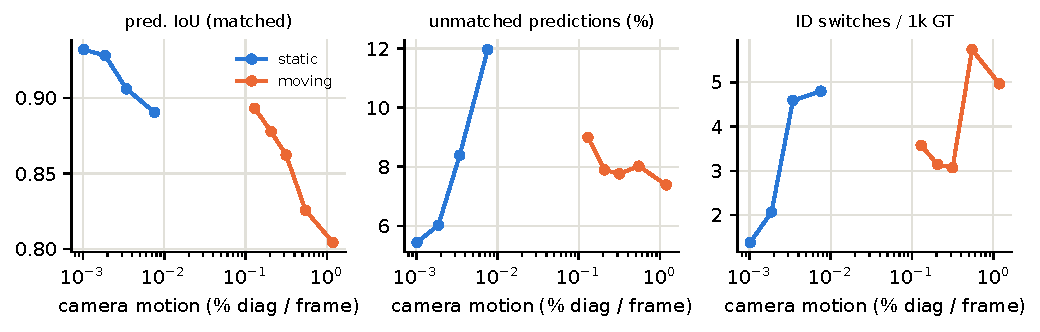
\includegraphics[width=0.92\textwidth]{fig_e3_binned}
\caption{Frame-level relations, binned by camera motion. Left: IoU of one-frame predictions with their matched
detections. Middle: share of predictions without a matching high-score detection. Right: ID switches per 1{,}000
ground-truth boxes. Bins mix sequences; claims in the text use within-sequence statistics.}
\label{fig:binned}
\end{figure*}

\textbf{Lost tracks.} The loss appears when a track has been lost and must be found again (Fig.~\ref{fig:lost}). The
prediction of a lost track is extrapolated over several frames, and its best IoU with any detection falls much faster
with a moving camera. After 9--16 lost frames, the best IoU is \vLostIoUMoving{} against \vLostIoUStatic{}, and only
\vLostMoving\% of the lost tracks are re-found, against \vLostStatic\% on static cameras. A track that is not re-found
comes back with a new identity, which is consistent with the larger AssA gap in E2. Fig.~\ref{fig:case} shows a frame of
MOT17-13 with the predicted and detected boxes.

Within the moving sequences, however, the camera motion accumulated during the gap does not predict recovery once the
gap length is fixed (median $\rho=\vLostRhoWithin$ over 30 gap lengths; pooled $\rho=\vLostRhoPooled$ is driven by gap
length). The penalty is therefore a property of moving-camera video as a whole rather than proportional to the size
of the motion.

\begin{figure}[t]
\centering
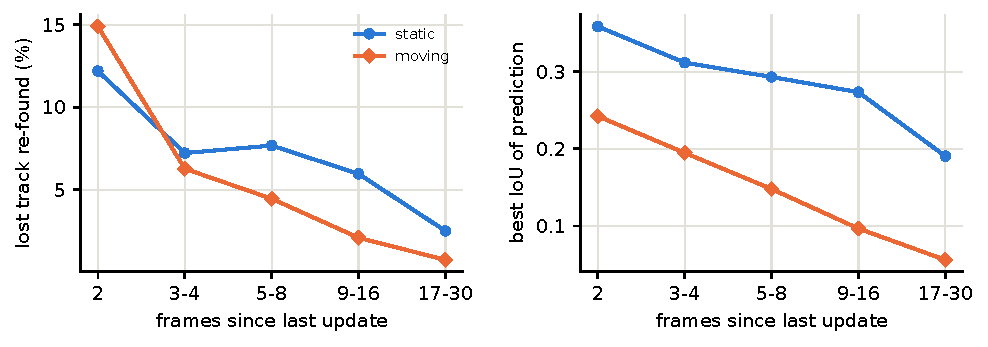
\includegraphics[width=\columnwidth]{fig_e3_lost}
\caption{Recovery of lost tracks. Left: share of lost-track predictions matched again. Right: best IoU between the
prediction and any high-score detection.}
\label{fig:lost}
\end{figure}

\begin{figure}[t]
\centering
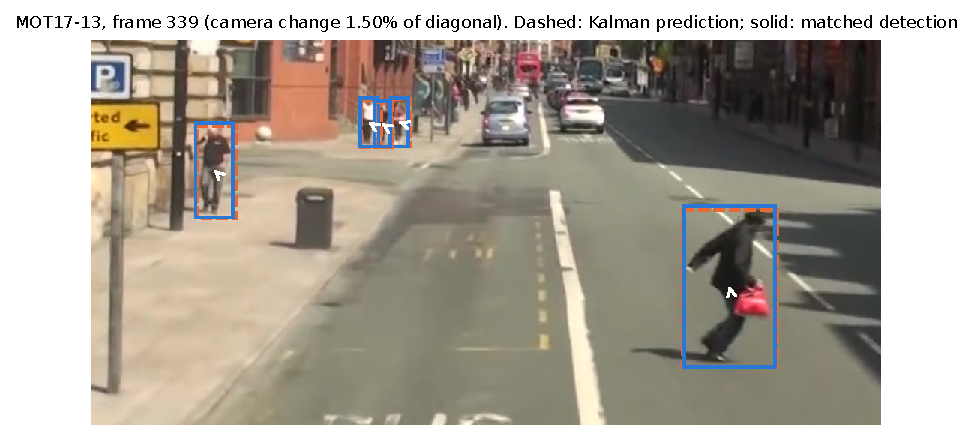
\includegraphics[width=\columnwidth]{fig_e3_case}
\caption{MOT17-13 (moving camera). Dashed: Kalman predictions; solid: matched detections; arrows: correction.}
\label{fig:case}
\end{figure}

\subsection{E4: Sensitivity study}\label{sec:e4}
We change one tracker parameter at a time around the official settings: the high-score threshold (0.4--0.7), the
matching threshold (0.7--0.95), the lost-track buffer (10--90 frames) and the standard deviation of the Kalman
\emph{process} noise ($\times0.25$ to $\times4$, measurement noise fixed). Scaling all noise terms of ByteTrack's filter
together leaves the Kalman gain, and therefore every prediction, unchanged, so only the process noise is varied. The
aim is to test whether the gap is stable, not to remove it.

Across all \vEfourN{} settings, moving cameras stay between \vEfourGapMin{} and \vEfourGapMax{} HOTA points behind static
cameras (Fig.~\ref{fig:e4}), and the AssA gap exceeds the DetA gap in \vEfourAssaCount{} of them. The thresholds and the
buffer hardly move the moving-camera result (HOTA \vEfourOtherMovMin--\vEfourOtherMovMax; gap
\vEfourOtherGapMin--\vEfourOtherGapMax). The Kalman process noise is the only parameter that acts mainly on the moving
group: making the filter trust its constant-velocity model more ($\times0.25$) lowers moving-camera HOTA to
\vKfQuarterMov{} while static cameras keep \vKfQuarterStat, and allowing more process noise ($\times2$) raises it to
\vKfTwoMov{} while static cameras drop to \vKfTwoStat. This asymmetry is consistent with E3: moving-camera tracks depend
on how quickly the filter accepts a change of image motion. Overall HOTA is highest at the official setting, so no
setting removes the gap without a cost elsewhere.

\begin{figure*}[t]
\centering
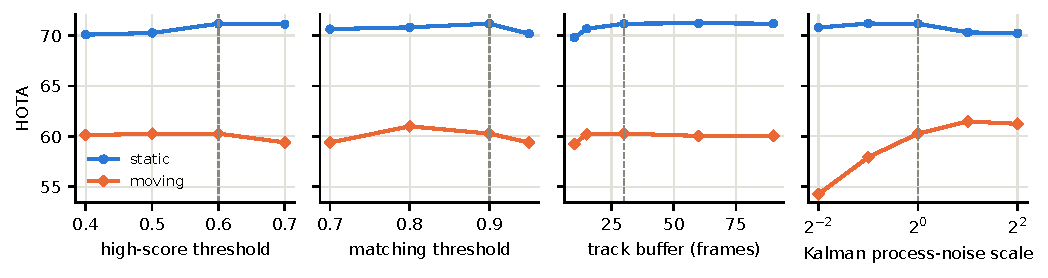
\includegraphics[width=0.92\textwidth]{fig_e4_sensitivity}
\caption{E4: HOTA of static and moving cameras when one parameter changes (dashed line: official value).}
\label{fig:e4}
\end{figure*}

% =====================================================================================================
\section{Discussion and Limitations}
Our results agree with the motivation of camera-motion compensation in BoT-SORT~\cite{aharon2022botsort}, but they
locate the problem more precisely: for ByteTrack on MOT17, camera motion hardly breaks frame-to-frame matching; it
mainly breaks the re-association of tracks after a gap. Three limitations apply. First, there are only seven sequences,
and the groups also differ in frame rate, viewpoint and lighting, so all results are correlational. Second, our camera
model is a 2-D similarity transform, which cannot describe parallax or the forward motion in MOT17-13. Third, the
analysis covers one detector and one tracker, and the sensitivity study changes one parameter at a time.

\section{Conclusion}
We reproduced ByteTrack on MOT17 half-val with the published MOTA and IDF1 and showed that the published numbers use
the code's matching threshold. Moving-camera sequences lose about \vGapHOTA{} HOTA points, mainly in association. Camera
motion degrades the Kalman prediction measurably, but the cost appears in the recovery of lost tracks, not in
frame-to-frame matching. The gap remains under all tracker settings we tested, and only the Kalman process noise changes it noticeably, which points to the motion model, rather than the detector or the matching thresholds, as the part to examine in future work.

\bibliographystyle{IEEEtran}
\bibliography{references}

\appendices
\section{Reproducibility}
{\footnotesize\raggedright
\textbf{Code:} \url{https://github.com/vanowarna/bytetrack-moving-camera}, release \texttt{v1.0} (commit \texttt{\repocommit}).
\textbf{Environment:} Python 3.11, PyTorch 2.7.1 (CUDA 12.8), locked with \texttt{uv}; ByteTrack \texttt{d1bf019};
TrackEval \texttt{12c8791}; NVIDIA RTX 5050 Laptop GPU (8\,GB).
\textbf{Run times:} detection \vDetMsFP{}\,ms per frame in FP16 (a few minutes for the 2{,}652 frames, run once and
cached); the live demonstration on MOT17-13 (detection, tracking, evaluation and video) takes about one minute.
\textbf{Seeds:} fixed; all tracking runs are deterministic given the cached detections.
\textbf{Commands} (all in \texttt{scripts/}; \texttt{make\_paper\_assets.py} then writes every number, table and figure):\par
\smallskip
\setlength{\tabcolsep}{3pt}\begin{tabular}{@{}ll@{}}
Data split & \texttt{make\_splits.py} \\
Table~\ref{tab:e1} (E1) & \texttt{run\_many.py -{}-configs "configs/e1\_*.yaml"} \\
 & \texttt{\phantom{run\_many.py} -{}-table e1} \\
Table~\ref{tab:seq} (E2) & \texttt{analyze\_e2.py} \\
E3, Figs.~\ref{fig:binned}--\ref{fig:case} & \texttt{run\_camera\_motion.py}, \texttt{run\_e3\_log.py}, \\
 & \texttt{analyze\_e3.py} \\
E4, Fig.~\ref{fig:e4} & \texttt{make\_e4\_configs.py}, \texttt{run\_many.py}, \\
 & \texttt{analyze\_e4.py} \\
\end{tabular}\par}

\IfFileExists{appendix_ai.tex}{\input{appendix_ai}}{}

\end{document}
